\documentclass{chi2009}
\usepackage{times}
\usepackage{url}
\usepackage{graphics}
\usepackage{color}
\usepackage[pdftex]{hyperref}
\usepackage{xspace}
\usepackage{graphicx}
\usepackage{caption}
\usepackage{subcaption}
\usepackage{listings}


\newcommand*{\system}{OGEN\xspace}
\newcommand*{\papertitle}{\system: Visualizing Physical Query Execution in a Relational Big Data Management System}
\newcommand*{\graph}{Physical Query Plan\xspace}
\newcommand*{\fragment}{Fragment Execution\xspace}
\newcommand*{\network}{Worker Communication\xspace}
\newcommand*{\overall}{Fragment Overview\xspace}

\hypersetup{%
pdftitle={\papertitle},
pdfauthor={Umar Javed, Thierry Moreau, Dominik Moritz, Adriana Szekeres},
pdfkeywords={},
bookmarksnumbered,
pdfstartview={FitH},
colorlinks,
citecolor=black,
filecolor=black,
linkcolor=black,
urlcolor=black,
breaklinks=true,
}
\newcommand{\comment}[1]{}
\definecolor{Orange}{rgb}{1,0.5,0}
\newcommand{\todo}[1]{\textsf{\textbf{\textcolor{Orange}{[[#1]]}}}}

\pagenumbering{arabic}  % Arabic page numbers for submission.  Remove this line to eliminate page numbers for the camera ready copy

\begin{document}
% to make various LaTeX processors do the right thing with page size
\special{papersize=8.5in,11in}
\setlength{\paperheight}{11in}
\setlength{\paperwidth}{8.5in}
\setlength{\pdfpageheight}{\paperheight}
\setlength{\pdfpagewidth}{\paperwidth}

% use this command to override the default ACM copyright statement
% (e.g. for preprints). Remove for camera ready copy.
%\toappear{Submitted for review to CHI 2009.}
\toappear{}

\title{\papertitle}
\numberofauthors{1}
\author{\alignauthor Umar Javed, Thierry Moreau, Dominik Moritz, Adriana Szekeres \\
\affaddr{Dept. of Computer Science, University of Washington} \\ \affaddr{Seattle, Washington, USA} \\
\email{\texttt{\{ujaved, moreau, domoritz, aaasz\}@cs.washington.edu}}
}

\maketitle

\begin{abstract}

We propose a visualization system for understanding and exploring query execution and data movement in a distributed database management system (DDBMS). Our tool provides insight into: (1) data flow between query fragments and between workers, (2) query execution and operator dependencies, (3) cluster utilization, (4) network utilization. Our tool, which we call \system, helps developers understand and improve query execution, and provides insight into common problems such as data skew or performance bottlenecks.

In particular, \system is built to inspect query execution in Myria\footnote{\url{http://myria.cs.washington.edu/}}, a distributed big data management system currently being developed in the UW CSE database group. Myria aims towards building a distributed database platform to provide \emph{big data management and analytics as a service} primarily for scientific applications.
The proposed visualizations can easily be applied to other DDBMS as well (e.g. Spark, Hadoop).

\end{abstract}

%\keywords{put author keywords here}

%\category{H.5.2}{Information Interfaces and Presentation}{Miscellaneous}[Optional sub-category]

\section{Introduction}

Database query performance is often unpredictable, specially when the DBMS is distributed. This requires database 
administrators to spend significant amounts of time and effort isolating and debugging the root cause of performance 
problems. These may include skewed data partitioning or run-time issues, such as resource contention or 
adverse network conditions.  

Our goal is to build a visualization tool designed to help a database administrator understand the data flow and run-time
performance during query execution in a Distributed Database Management System (DDBMS). Using our tool, the
database programmer or administrator could quickly discover run-time bottlenecks as well as problematic data skew issues, 
saving them significant guesswork and programming effort to identify the appropriate logs to analyze. Our visualization tool
is called \system, which uses profiling logs from Myria \cite{myria} as the prototype DDMS. Myria is a distributed 
database platform that provides \emph{big data management and analytics as a service} primarily for scientific applications.
Myria takes queries in high-level query languages, such as SQL, translating them into physical query plans and finally executing
them in parallel. Currently, Myria does not offer a visualization tool designed to show the physical query plan, job execution and network 
communication between distributed workers. \system allows the programmer/database administrator to visualize the following aspects
of query execution.

\begin{itemize}

\item An interactive visualization of the physical query plan. The physical query plan in Myria is composed of
a DAG of fragments, where each DAG link represents communication between workers, possibly over the network. 
\system displays this DAG in an interactive fashion with clickable elements for fragment nodes and communication links. 
This DAG also represents a high-level data flow in the DDBMS. 


\end{itemize}


% Umar

% What is myria, how does it work (look at report from last quarter but shorter), which query languages are supported
% motivation
% questions (inspiration: https://docs.google.com/a/uw.edu/document/d/1Syn65bu_p6S4RQETaozsleYcRBauQJ7IduYrctS1wrw/edit?pli=1#)
% why is a visualization a good way to answer the questions
% so far the only performance debug mechanism is runtime
% contributions
% explain difference between execution and data skew

% \item Questions: find data/execution skew, identify performance bottlenecks, visualize data flow in the system (elaborate on each point)...


\section{Related Work}

Twitter developed Ambrose\cite{ambrose}, a platform for visualization and real-time monitoring of MapReduce data workflows. They offer three different views to show associated jobs, job dependencies and progress. Ambrose has been released as open source. Ambrose, however, is not suitable for our needs as the abstraction level of jobs is too high and does not capture single operators.

Google's Dapper\cite{sigelman2010dapper} is a distributed systems tracing infrastructure and offers fine grained tracing of calls in Google's distributed systems. They also proposed an interface for visualizing traces. Similarly, X-trace\cite{fonseca2007x} was developed as a framework to trace which events cause what other events in a distributed environment. recently, there has been work on visualizing event traces collected in X-trace\footnote{\url{https://github.com/brownsys/X-Trace/tree/master/src/webui/html/interactive}}. Due to the importance of these kinds of debug facilities, Twitter closely modeled Zipkin\cite{zipkin} after Dapper and X-trace and released it as open source.

Dapper and X-trace focus on how data flows through a distributed system. In \system the visualization focuses on the operators and how the data flows through them. This orthogonal view is better suited for debugging performance bottlenecks in DDBMS and also scales to a larger number of events. Furthermore, in contrast to  we offer different abstraction levels, which enables users to find problems faster and handle larger amounts of profiling data. Also, \system is specifically designed to help developers understand query execution in distributed database system like Myria as opposed to general traces in distributed systems.

Tools to visualize query plans for example in SQL Server, as used to improve performance for the SDSS Sky survey\cite{szalay2002sdss}, focus on optimizing queries and not query execution and have no visualization of data flow, which is necessary to optimize physical query execution.

\section{Approach}
\label{sec:approach}

% Adriana

The first step in designing \system was to identify the possible causes that
could affect the execution performance of the query. After we identified
several such causes, that we will enumerate below, we leveraged visualization
techniques that we found fit to allow developers/programmers to get insight
into how the query was executed on the available resources and quickly
identify the source(s) of the performance penalty.

We found that the performance of the query might be affected by the following
factors, which greatly influenced the design of our visualization tool:
\begin{itemize}
   \item \emph{Wrong/unoptimized physical query plan.} We manually analyzed
several physical query plans and discovered that some queries were poorly
optimized. This led us to design a view that allows interactive exploration of
the physical query plan (mapped to a graph of query operators).
   \item \emph{Stragglers, tail latency, expensive query operators, poor
scheduling.} Our targeted systems are \emph{distributed} databases. Therefore,
as the query is executed in a distributed environment, the query coordinator
has to wait until all the workers finish executing their assigned tasks. To
give insight into how the tasks are distributed and executed at each workers,
we designed a view that shows the cluster utilization over time and at each
worker.
   \item \emph{Poor data partitioning, data skew.} Network traffic can cause
serious delay when executing a distributed query. Due to poor data
partitioning, workers might need to send unnecessary big amount of data between
each other. We designed a view that allows the developer/programmer to analyze
the data traffic generated while executing the query.
\end{itemize}

% Why did we choose the visualization
% How it is implemented
% explain how events and logs are used to create the raw data for vis

\system's architecture (Figure~\ref{fig:arch}) consists of a back-end,
used as a plug-in interface for the distributed database system targeted, and a
front-end which implements the views described above. The front-end and
back-end of \system are highly decoupled so that the visualization can be used not only with
Myria but also with other systems such as Spark or Hadoop. In
Section~\ref{sec:back} we illustrate how we implemented log collections and
aggregation in Myria.

\subsection{Back-end}
\label{sec:back}

The task of the back-end is to log when operators are called, when the call returns and when data is sent to another worker. Using this data and simple transformations, we can obtain the information necessary to create the visualizations to answer the questions in Section~\ref{sec:approach}.

There are two possible approaches that we explored to collect event logs that can be used to extract spans and other performance related data necessary for the visualization. First, events could be logged to files using a standard logging tool and then collect the files on one node using remote copy. Once the logs are on one machine, the logs can be parsed and the data can be transformed into the desired format.

We switched to a different approach as shown in Figure~\ref{fig:arch} where logs are written directly into the worker's database. When the front-end requests the data, the master executes a query that collects the data and streams the results directly to the requesting client. Logs are thus tuples in a relation and no longer separate in files and in a custom format. Despite being more reliable, faster and using the same logic that Myria already implements, we are able to write queries to aggregate, filter and transform the collected data.

For example, the data for how many workers are working on a certain fragment as described in Section~\ref{sec:fragments} is generated from the event log using a query to select only events for the root operators (the operators that have no parent in the same fragment) in each fragment and a custom map function that carries state. The state is an integer that is incremented when the operator is called on a worker and decremented when the operator returns.

\begin{figure}[ht]
  \includegraphics[width=\columnwidth]{images/viz_arch}
  \caption{Overview of the log collection and transformation architecture. Raw event logs are collected on each worker. The data is stored in relations. To download the data, a query has to be executed.}
  \label{fig:arch}
\end{figure}

We highly suggest that developers use the second approach when porting \system to a new DDBMS.

\subsection{Front-end}

The Myria web front-end server is written in Python and runs on Google App Engine\footnote{\url{https://developers.google.com/appengine/}}. \system's user-interface (UI) is embedded into Myria's web front-end. We build \system's UI using D3\cite{2011-d3} to deliver an interactive visualization experience to the user. D3 is a JavaScript framework for data visualization on the web. We used visualization techniques such as \emph{focus+context}\cite{furnas1986generalized} that possible to implement conveniently using D3.

\system's front-end gets data from the Myria server as JSON and CSV files. JSON objects are used to describe the physical queryplan. CSV files contain logs on query execution at the fragment and operator level as well as data exchange between workers at different stages of the query execution.

\system's web UI is divided into two components: (1) the browser panel which provides a visualization of the \graph, and (2) the performance panel which provides some insight into an element selected in the browser view. The browser panel contains a view of the \graph, rendered as a graph. The user can navigate the \graph by expanding query fragments into the operators that compose it. The user can chose to select a fragment of interest which will render a \fragment visualization of the selected fragment in the performance panel. Alternatively, the user can select an fragment-to-fragment edge in the \graph thus rendering a \network visualization of the selected edge in the performance panel. If no elements are selected in the \graph view, an \overall visualization is rendered in the performance panel, displaying the aggregate worker utilization over time for each fragment.

The following subsections describe each one of the four views offered by \system's web UI.

% Thierry

\subsubsection{Physical query plan view}

% Thierry

% Figures
% 1: Graph with back-edge
% 2: Large Graph expanded vs. large Graph reduced vs. large graph expanded -1


\begin{figure}[ht]
  \centering
  \begin{subfigure}[b]{0.49\columnwidth}
    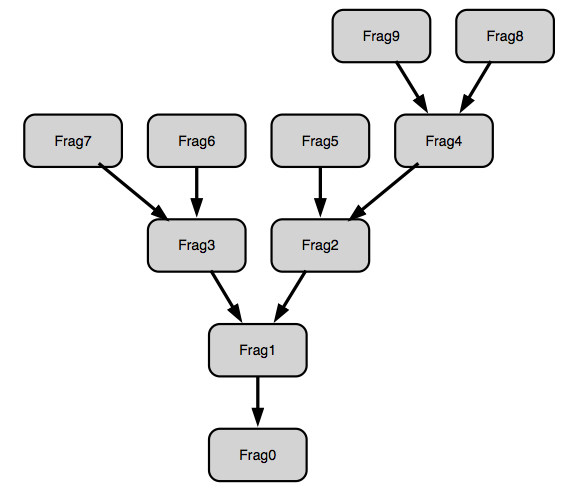
\includegraphics[width=0.8\columnwidth]{images/graph_collapsed}
    \caption{Large query plan collapsed.}
    \label{fig:graph}
  \end{subfigure}
  \begin{subfigure}[b]{0.49\columnwidth}
    \includegraphics[width=0.8\columnwidth]{images/graph_expanded}
    \caption{Expanding Fragment 2 reveals its operators.}
    \label{fig:graph_expanded}
  \end{subfigure}
  \caption{The \graph view is used by \system to help the user browse performance visualizations.}
  \label{fig:graph}
\end{figure}


The \graph view as pictured in Figure~\ref{fig:graph} allows the user to selectively browse different performance visualizations tied to a given query execution. The \graph view provides as the name indicates, a visualization of the physical query plan. A query plan is an ordered set of steps used to access data in database management systems. The physical query plan is represented by a graph where each node represents a query fragment, and each link represents inter-worker communication from one query fragment to the next. Each query fragment is a collection of query operators. One can think of a query fragment as a job unit that gets scheduled on a cluster of machines. Consequently transitioning from one query fragment to another generally leads to all-to-all communication between worker nodes on the cluster. 


The user can perform three classes of actions that will render a new visualization in the performance panel:
\begin{itemize}

    \item \textbf{Empty selection:} by default if no fragments or edges are selected in the \graph view, an \overall visualization is rendered in the performance panel. This visualization displays the aggregate worker utilization over time for each fragment and provides cluster utilization data at a glance.
    \item \textbf{Fragment selection:} when selecting a fragment, a \fragment visualization gets rendered in the performance panel. The \fragment visualization provides aggregate cluster utilization information complemented by per-worker task schedules. When a fragment is selected, the operands inside of the fragment in the \graph view are color-coded to allow the user to easily match each task in the per-worker task schedule in the performance window with the corresponding query operator in the browser window.
    \item \textbf{Edge selection:} upon selecting one or more fragment-to-fragment edges, a \network visualization gets displayed, providing information on inter-worker communication from one query fragment to the next.

\end{itemize}

\textbf{Graph Rendering:} We use D3 \cite{d3} to render the \graph graph, which allows us to support various interactions and transistions. We use GraphViz \cite{Ellson01graphviz} in the backend to generate graph layout information. GraphViz allows us to generate graph layouts that are optimized to minimize area footprint. The layout information is then fed into a D3-based rendering engine which supports various interactions and animations techniques.

\textbf{Graph Navigation:} A query plan can be arbitrarily large. Thus we offer two mechanisms that facilitate exploration of the graph for the user: (1) expanding/reducing fragments and (2) zooming. The first mechanism can reduce the size of a graph by a constant factor by collapsing operators that compose a fragment into a single fragment node. The user can click once on a collapsed fragment to expand, and click once on an expanded fragment to collapse it. Expanding or reducing a node can cause large changes in the graph layout as GraphViz changes the graph layout to minimize overall area. This graph reshuffeling is illustrated in Figure~\ref{graph} where expanding Frag2 causes the layout to change. To address these layout changes, we implemented transitions to allow the user to track the fragments as those get reshuffled. The second mechanism that facilitates exploration of the graph for the user is zooming. This feature was implemented in D3 and allows the user to quickly jump from one part of the graph to the next, by zooming in and out of the graph view.

\textbf{Tooltip Information:} \todo{write me}


\subsubsection{Fragment execution view}
\label{sec:fragment}

% Adriana

The \fragment view comprises two charts: the utilization chart and the
operators chart. The utilization chart (Fig.~\ref{fig:utilization_chart}) shows on
how many workers a fragment is running over time. The chart is used to
quickly reveal any patterns in the schedule, like tail latency, long periods of
idleness, etc. We implemented a small brush (at the top of the figure) that
allows the user to zoom-in and further analyze the problematic area.

\begin{figure}[ht]
  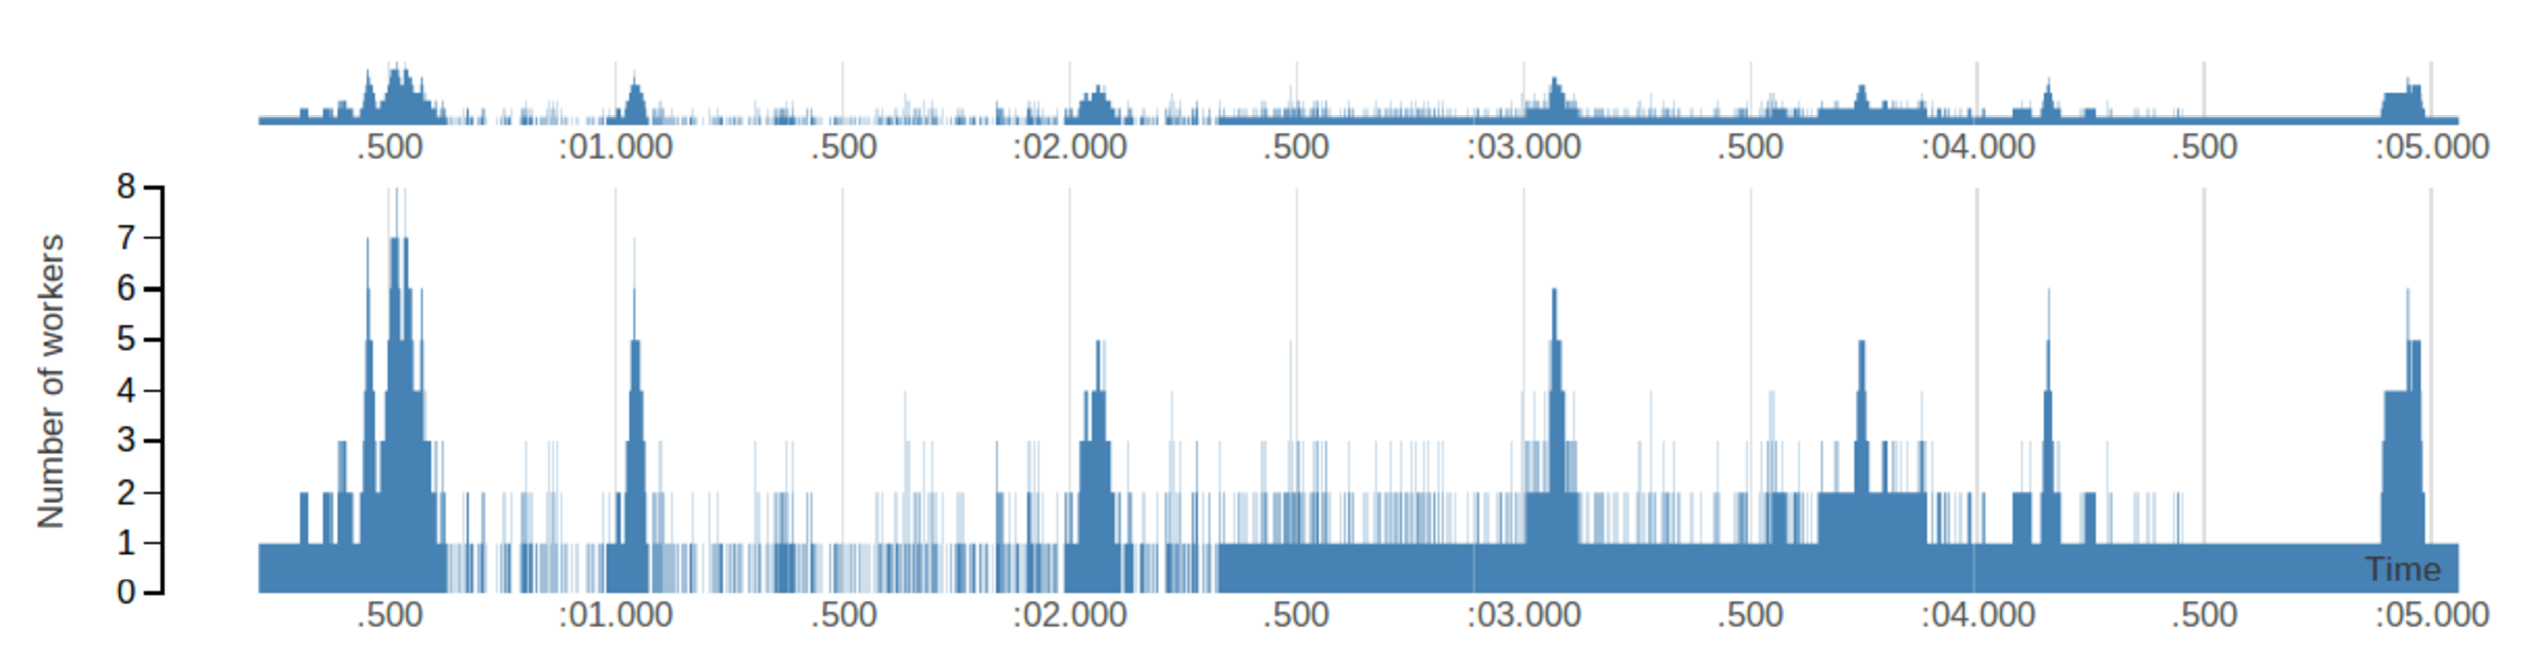
\includegraphics[width=\columnwidth]{images/utilization_chart}
  \caption{The utilization chart. }
  \label{fig:utilization_chart}
\end{figure}

The utilization chart also implements a brush that allows the user to further
analyze the query execution by displaying the schedule of each of the worker
nodes, in the operators chart (Fig.~\ref{fig:operators_chart}). The per-worker
schedule shows what operators the worker executed and for how long.


\begin{figure}[ht]
  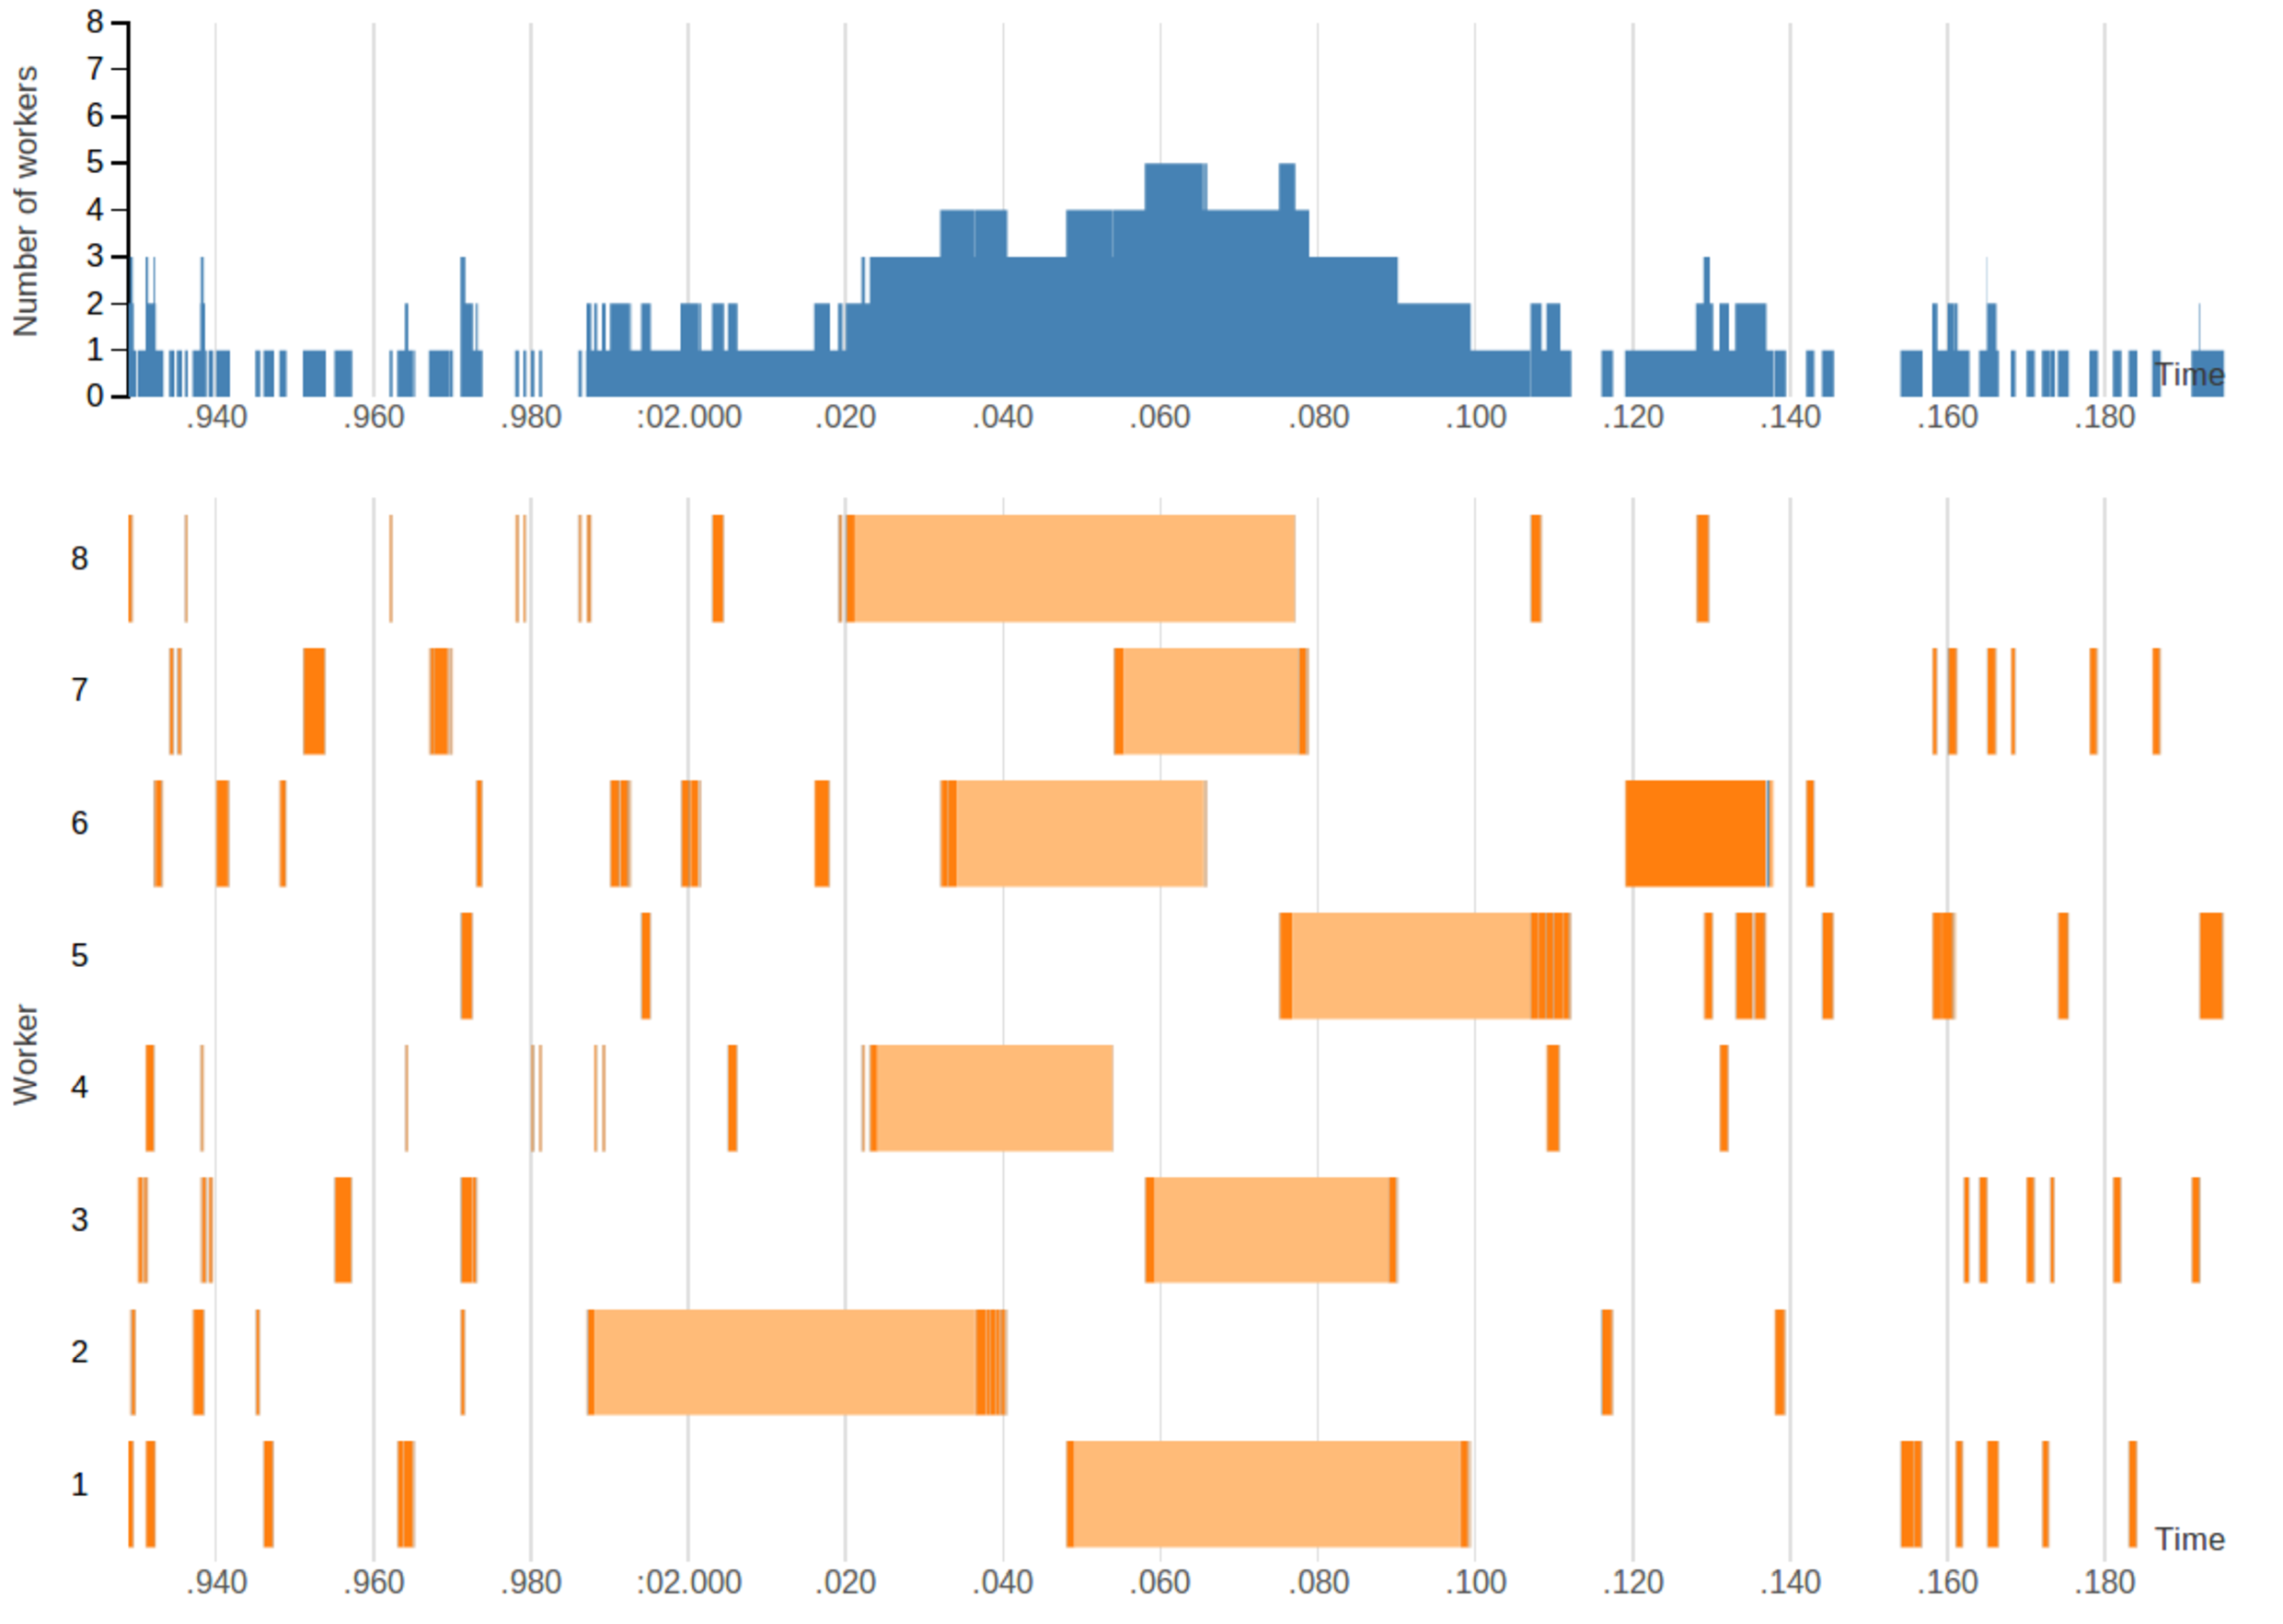
\includegraphics[width=\columnwidth]{images/operators_chart}
  \caption{The operators chart.}
  \label{fig:operators_chart}
\end{figure}

% use the word spans when referring to events with duration (used in dapper)

\subsubsection{Overview over all fragments}
\label{sec:fragments}

% Dom

The \overall shows small multiples of the utilization chart as described in the previous section.
Execution skew can be spotted in this view. Furthermore, the user can compare the fragments and find
correlations between the execution of different fragments. This view helps the user navigate to the
right fragment and is not intended to offer further inside into the causes or performance problems.

% Write about small multiples view

\subsubsection{Worker communication view}

% Umar

\todo{write me}

\section{Evaluation}

We used \system to examine real world database queries that ran on Myria. We base our analysis on the different visualizations that were generated by \system and present examples where the \system helped us better identify (1) data skew, (2) execution skew, (3) performance bottlenecks. 

We explore a simple join query we performed on one million tuples extracted from the Twitter user graph. This query joins Twitter followers and followees by user ID. The query can be written in SQL as expressed below.

\begin{lstlisting}
SELECT *
FROM twitter S, twitter R
WHERE S.follower = R.followee
\end{lstlisting}


\begin{figure}[ht]
  \centering
  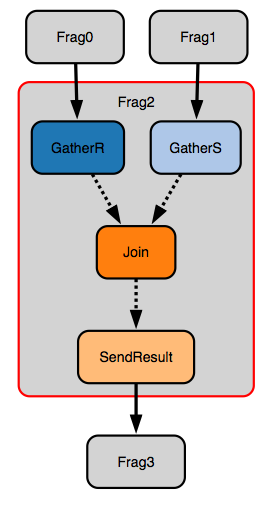
\includegraphics[width=0.4\columnwidth]{images/graph_join}
  \caption{This view shows the \graph for a join.}
  \label{fig:join}
\end{figure}


The resulting \graph visualization is displayed in Figure~\ref{fig:join}. The user will navigate the \graph visualization in the browser panel in the next case studies to identify several performance symptoms.


% How it helps
% Examples

% Thierry + Dom

\subsection{Case 1: Identifying Performance Bottlenecks using the \overall}

%dom

\subsection{Case 2: Identifying Data Skew using the \network View}

\begin{figure}[ht]
  \centering
  \begin{subfigure}[b]{0.49\columnwidth}
    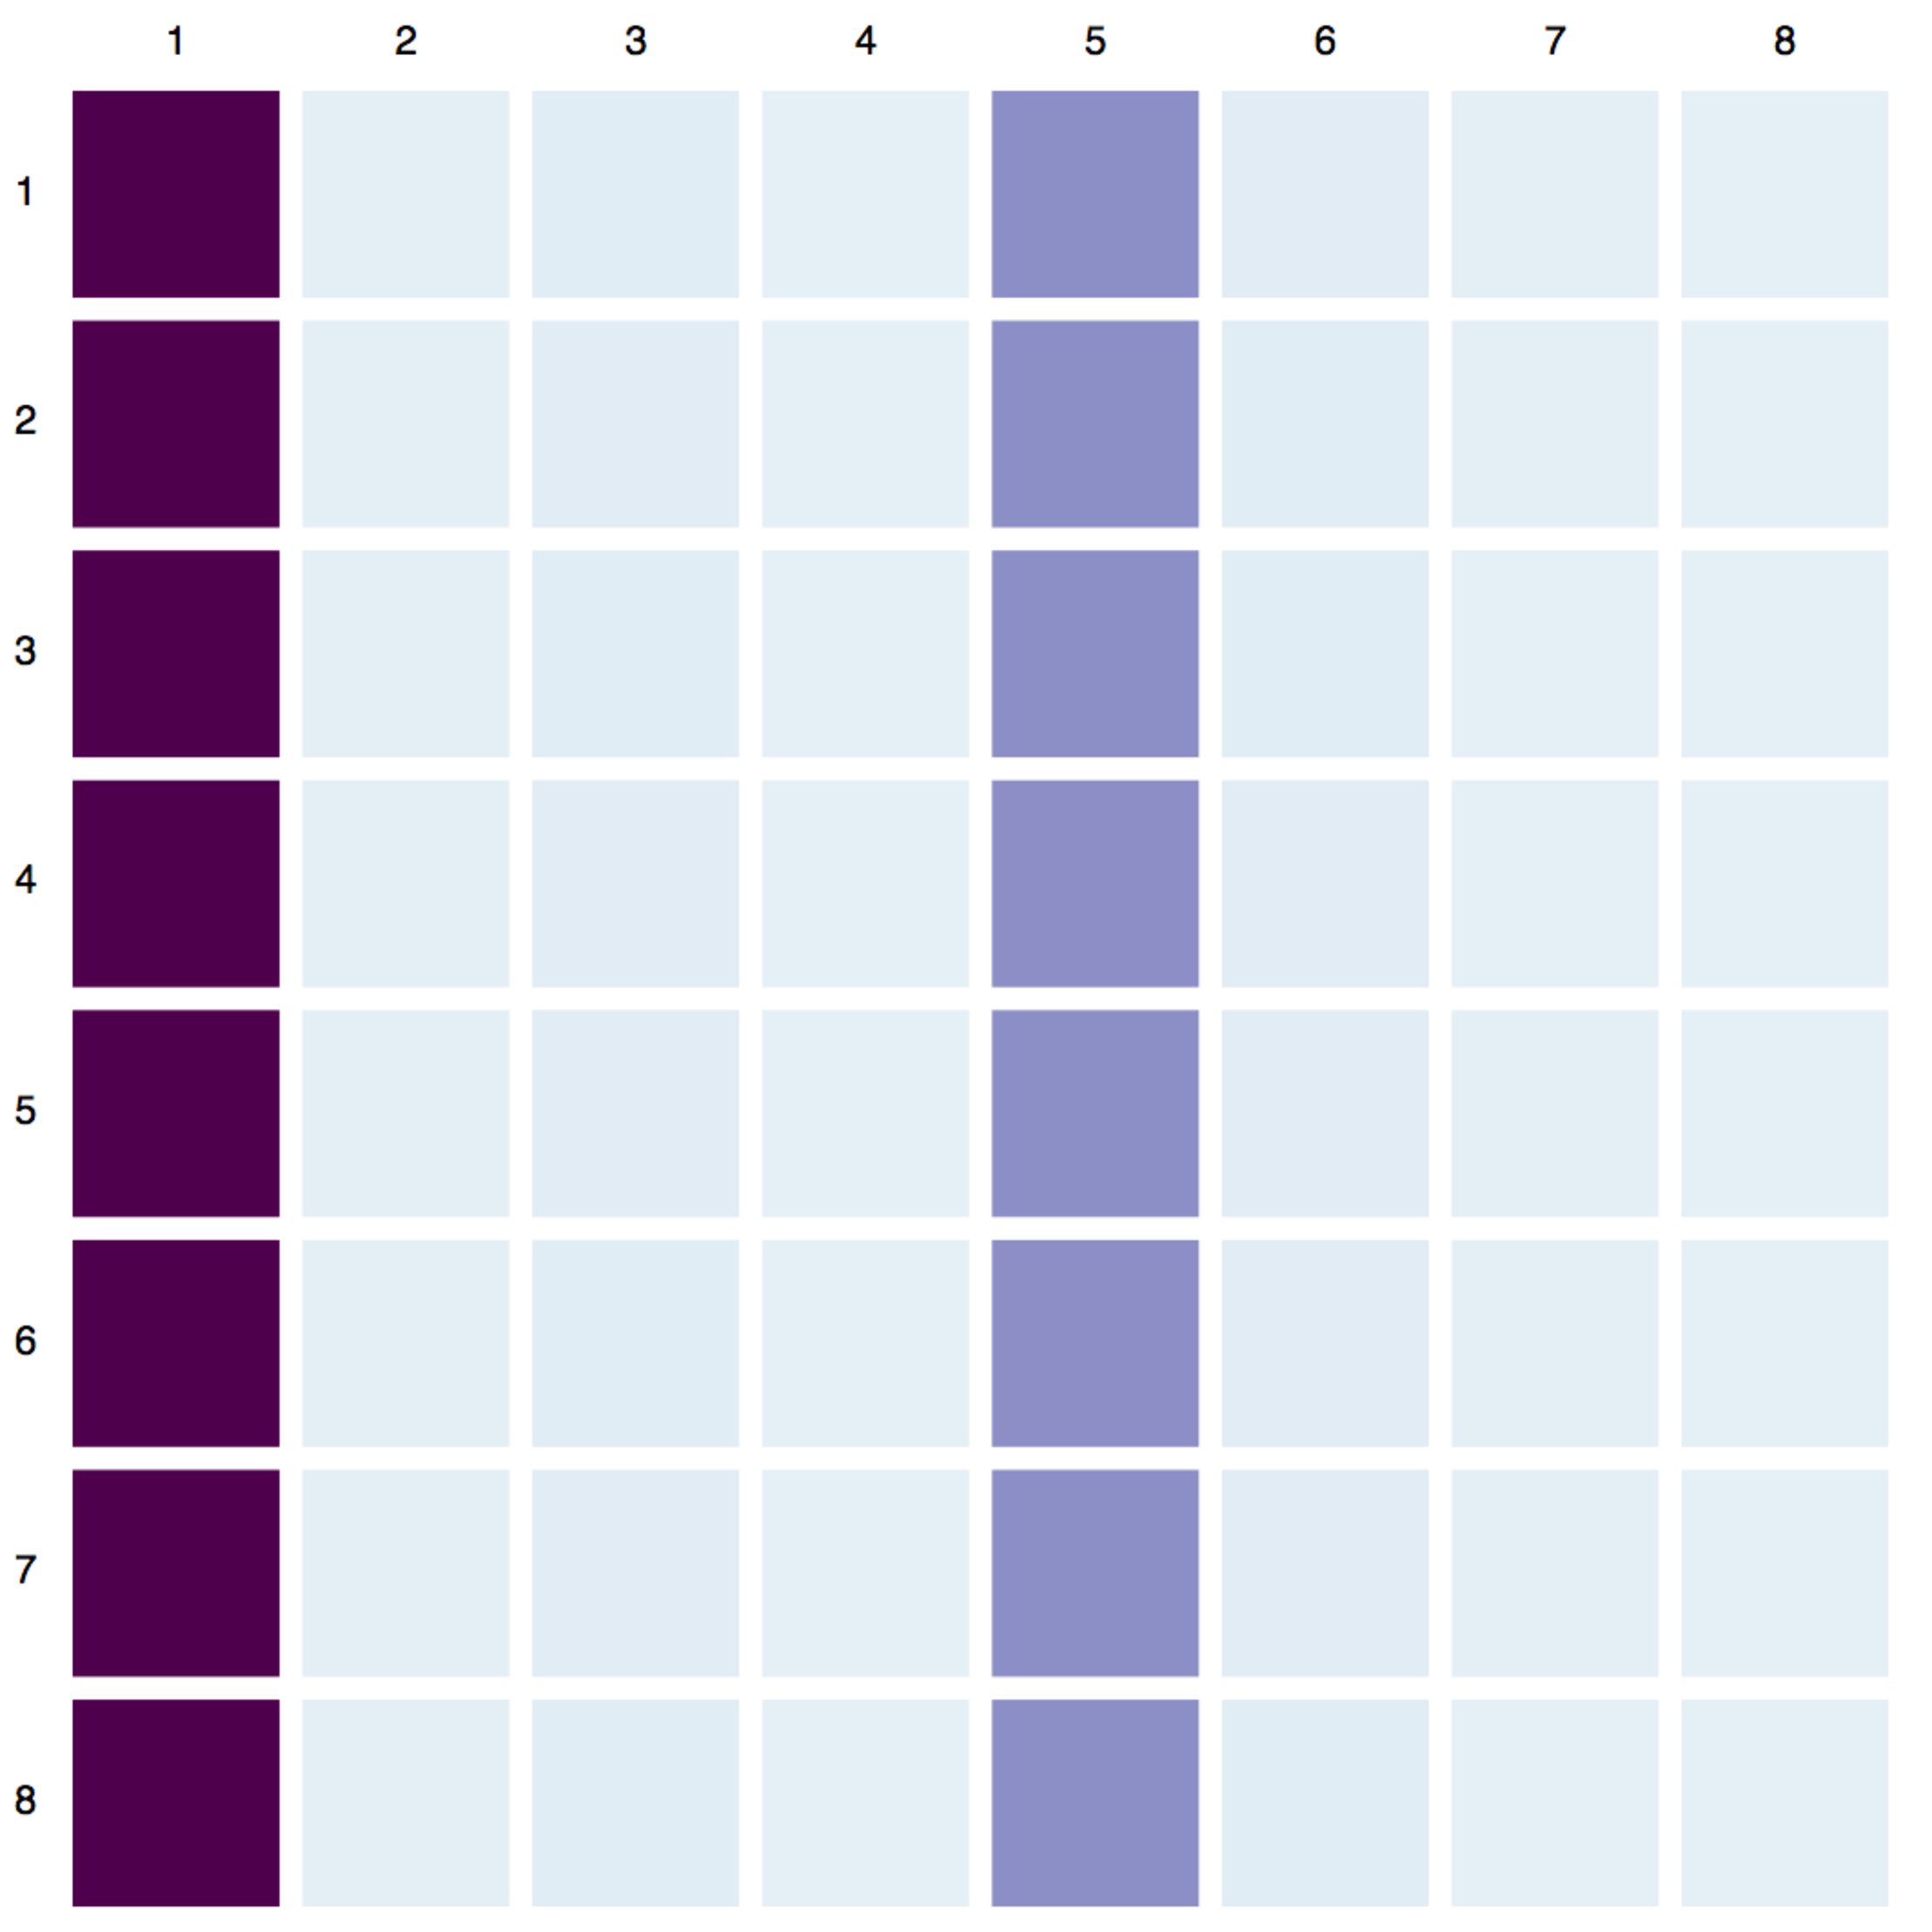
\includegraphics[width=\columnwidth]{images/skew}
    \caption{Data skew.}
    \label{fig:skew}
  \end{subfigure}
  \begin{subfigure}[b]{0.49\columnwidth}
    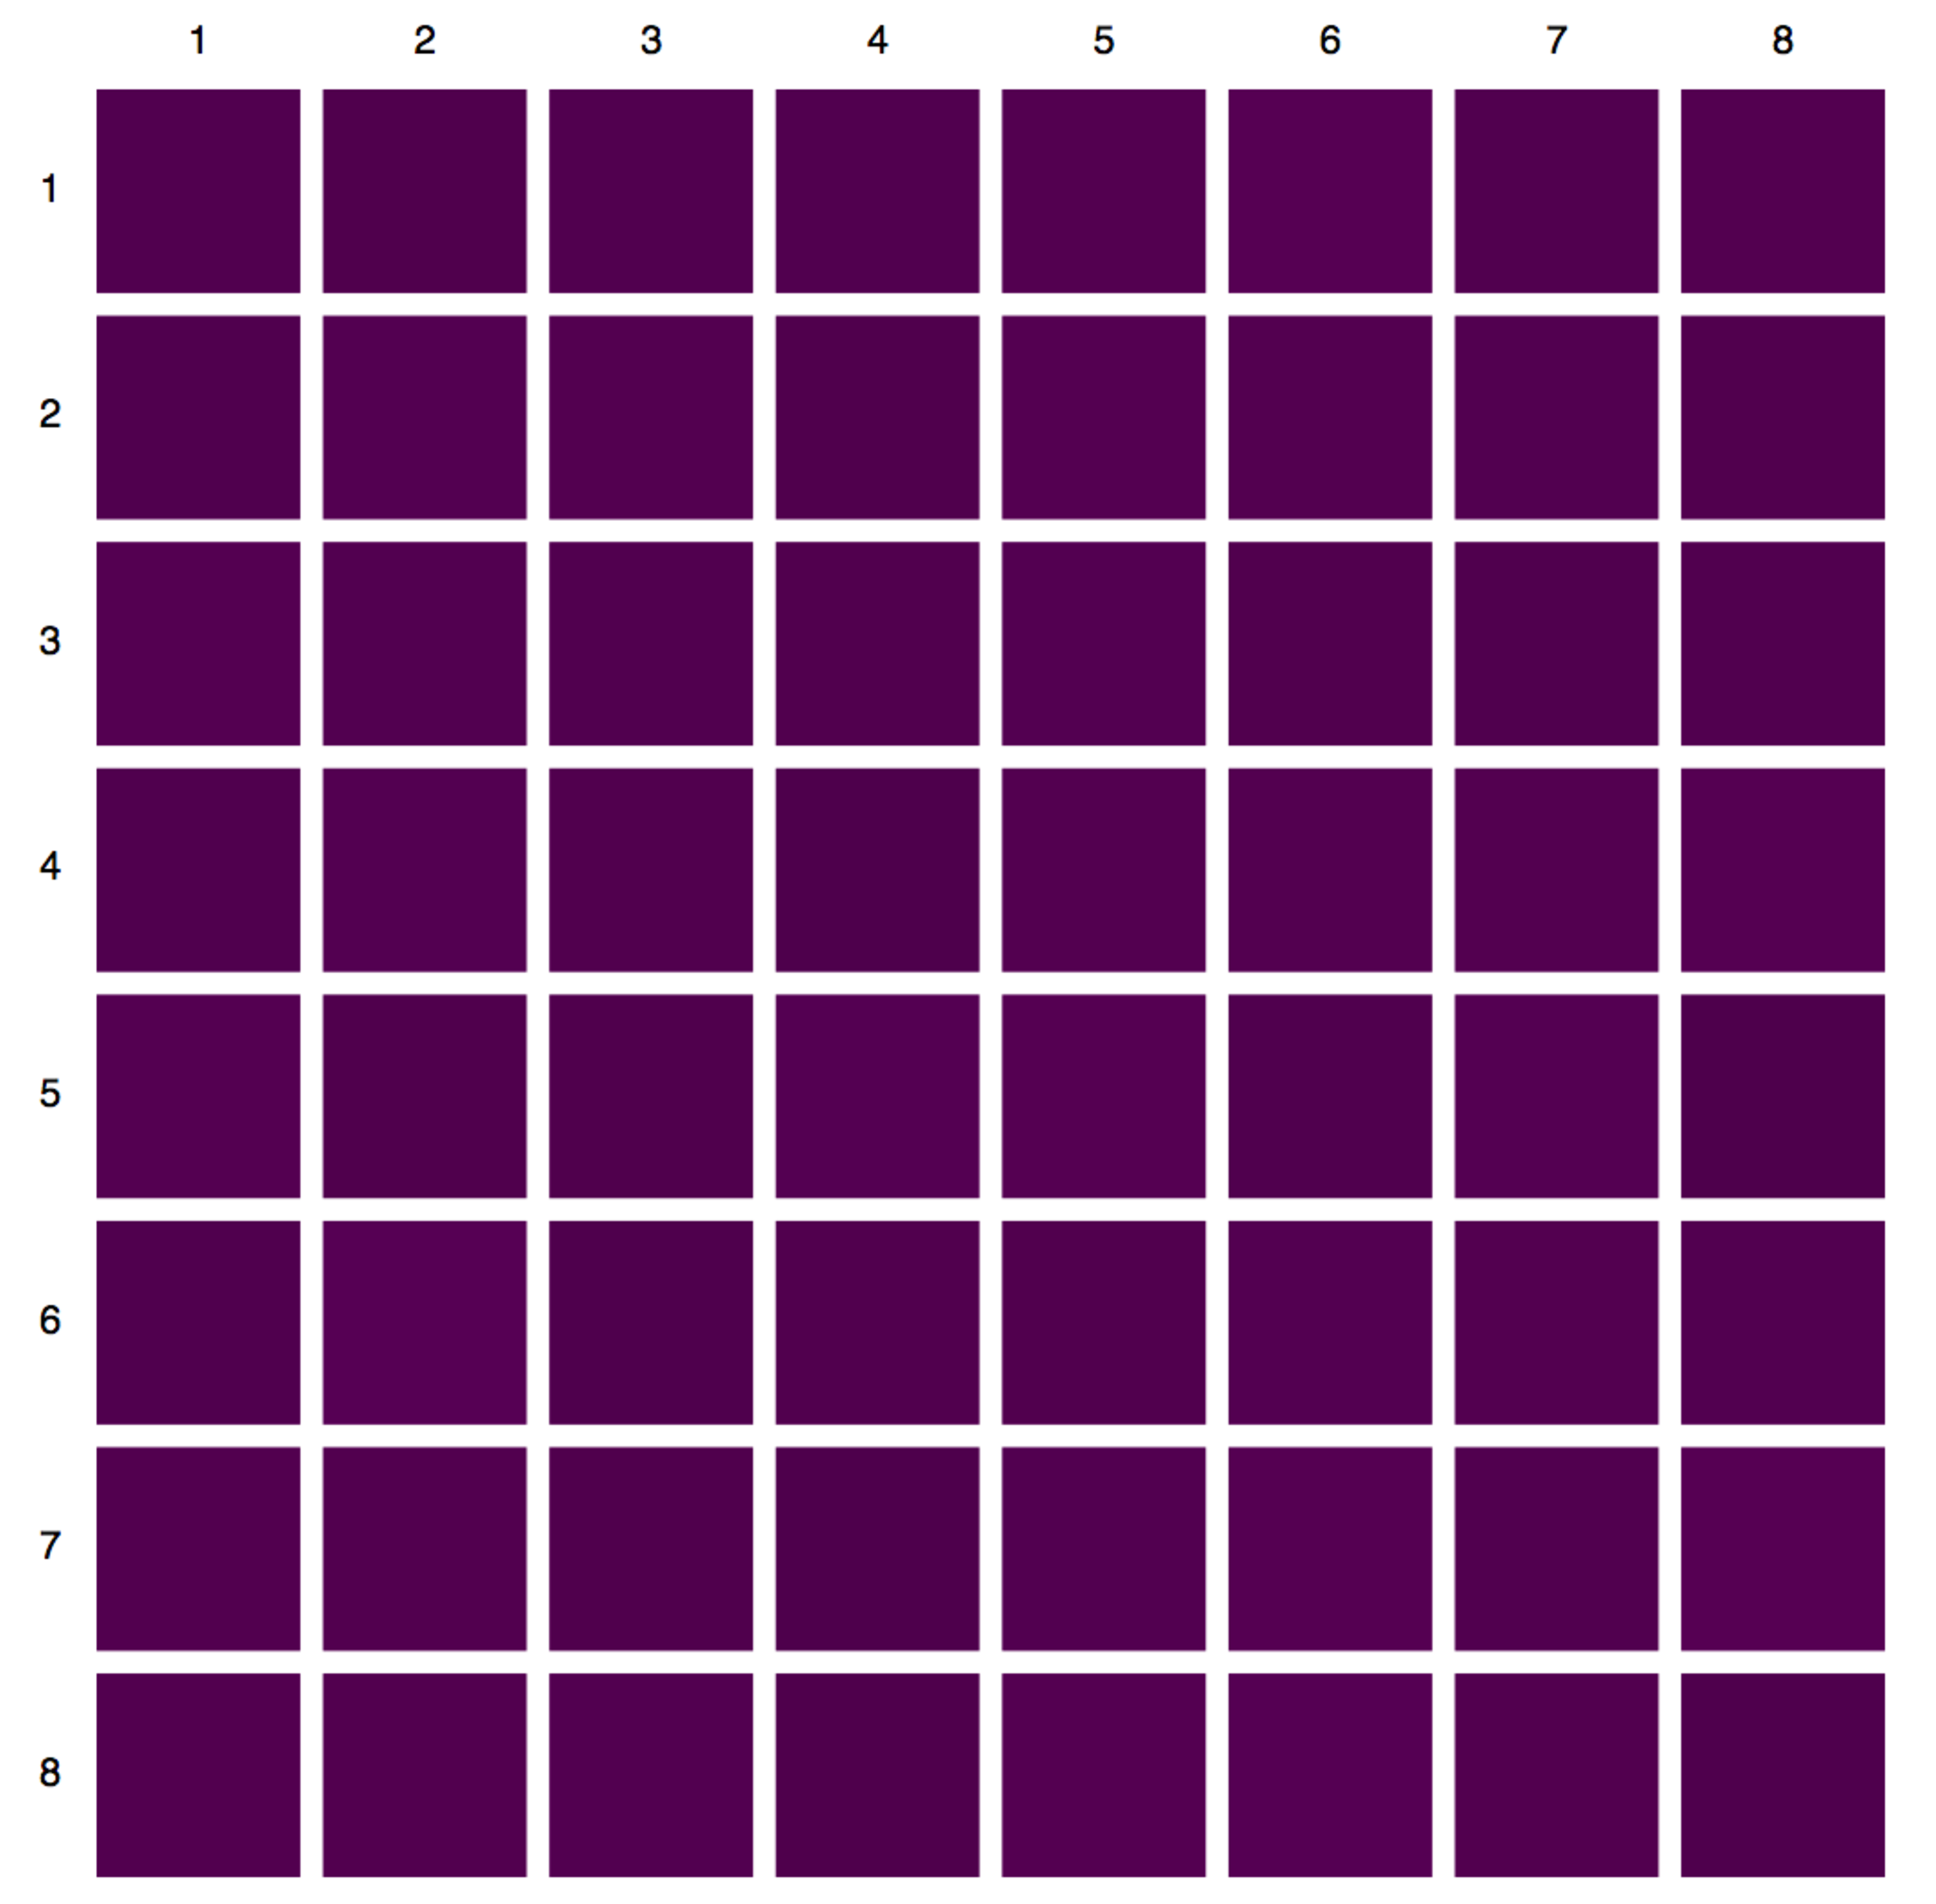
\includegraphics[width=\columnwidth]{images/no-skew}
    \caption{No data skew.}
    \label{fig:no-skew}
  \end{subfigure}
  \caption{The network view shows a distinctive pattern when there is data skew. Figure~\ref{fig:skew} shows that most tuples are sent to worker 1 and 5 (origin: row, destination: column).}
  \label{fig:network}
\end{figure}

The \network visualization at a glance shows how much data was sent between workers by one query fragment to the next. The two \network views in Figure~\ref{fig:no-skew} and Figure~\ref{fig:skew} were obtained by selecting the Frag0$\rightarrow$Frag2 and Frag1$\rightarrow$Frag2 edges respectively in the \graph view. Figure~\ref{fig:network} displays aggregate data communication between workers. In Figure~\ref{fig:no-skew} the amount of data sent from each worker to every other worker is balanced as opposed to Figure~\ref{fig:skew} where one can see that the volume of data sent to worker~1 and worker~5 outweights data sent to the other workers in the system. This apparent data skew could be caused by partitioning issues.

\subsection{Case 3: Identifying Execution Skew using the \fragment View}

\begin{figure}[ht]
  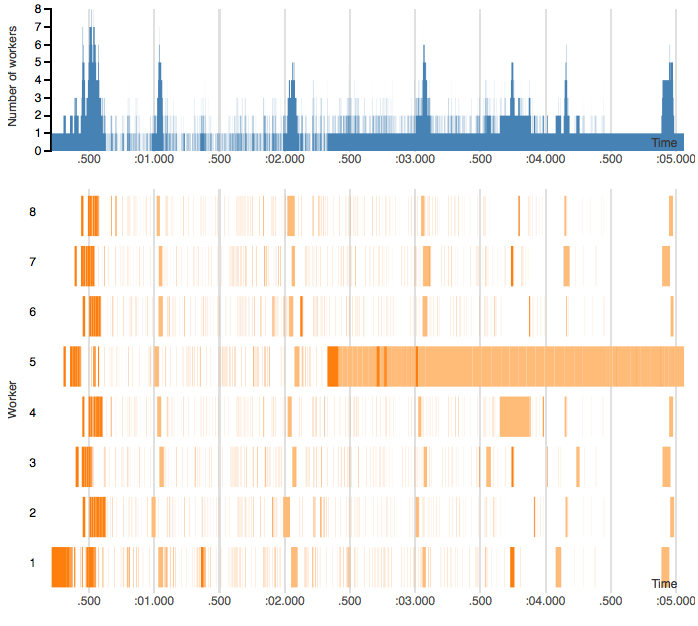
\includegraphics[width=\columnwidth]{images/execution_skew}
  \caption{This \fragment view shows heavy execution skew on worker~5.}
  \label{fig:exec_skew}
\end{figure}

The \fragment visualization allows the user to dive down into query execution details at the worker level. The \fragment view in Figure~\ref{fig:exec_skew} was obtained by selecting Frag2, which is the fragment that performs the join, in the \graph view. The user can observe at a glance that certain workers produce much more data as a result of the join execution. Particularly, we saw in Case 2 Figure~\ref{fig:skew}, that tuples sent to Fragment 2 from Fragment 1 were heavily skewed towards being sent to worker~1 and worker~5. In Figure~\ref{fig:exec_skew}, the user can now see that as a result of the join, worker~5 ends up producing most tuples that have to be written back to disk. The color scheme used for each worker schedules in the \fragment view is color-coded to match the operators in Figure~\ref{fig:join}. Consequently, one can quickly observe in the \fragment view that worker~5 is busy sending join results from t=2.5s to t=5.0s, which differes from the rest of the workers. Using similar reasoning, one can conclude that worker 5 presents a performance bottleneck in the execution of the query on Myria. Perhaps the user can modify the way the input data set gets partitioned. Alternatively she could change the number of workers allocated for the job. 

\subsection{Discussion}

All in all, \system allows the user to get much more insight into the execution of a query than what was available before, i.e. text-based performance logs, and runtimes. Being able to navigate performance data using a simple interface can indeed facilitate the task of a developper who is designing Myria's back end, or a Myria user who is writing complex queries to process large amounts of data. That said, \system can only help the user visualize query execution performance, but won't necessarily point the user to what she needs to do to improve performance of her query execution. 


\section{Conclusion}

% Adriana

% Capabilities and Limitations

\todo{write me}

\section{Future Work}

A focus of the current implementation is on scalability to many workers and long running queries. More aggregations have to be done by the database itself. Most importantly, in the fragment visualization that shows spans for all events we should limit the data that is being downloaded and rendered to what the user can see. With the architecture as explained in Section~\ref{sec:back}, we are able to express these filter conditions as queries.

Besides performance improvements, we plan to integrate X-trace and its visualization to offer the orthogonal view and allow users to trace how tuple batches flow through the operators and between operators. Combined with the visualizations described in this paper, it will form a powerful debugging tool that will help us to better understand and improve query execution.

\bibliographystyle{abbrv}
\bibliography{paper}

\end{document}
